\chapter{Introduction}
  talk about self-reported pain and intensity estimation
  why didn't I do any intensity estimation stuff?
  Regression is difficult??? Classification is a different thing.
  take about the fact that you are doing one frame and a time and
  other methods might be better becuse they can do sequences.
  \section{Problem Space}
    The human face is most likely one of the most researched objects in image analysis
    and computer vision \cite{S.ZafeiriouA.PapaioannouI.KotsiaM.A.Nicolaou}.
    It has wide ranging applications from Human
    Computer Interaction (expression recognition) to law enforcement (face recognition).
    Its study necessitates the development of a wide range of machine
    learning and computer vision research.

    Facial Action Unit detection FAU \cite{Corneanu2016} is chosen in this work due
    to it's popularity and available benchmarks.
    The Facial Action Coding System (FACS) developed by Ekman and Friesen,
    provides a systematic way to study any kind of facial expression,
    by representing them as a combination of individual facial muscle actions
    known as Action Units (AU). Automating the process of detecting AUs is difficult
    because they have non-linear interactions and often occur in very low intensities.

    There exist many datasets containing images and videos of faces and it is a general
    observation that unlabelled images are far more abundant than labelled ones.
    In particular in the areas of expression recognition where painstaking work
    must be carried out to obtain the ground truth expressions for an image or set of
    frames in a video. This situation is one of the motivations for this project.

    \begin{figure}
     \centering
     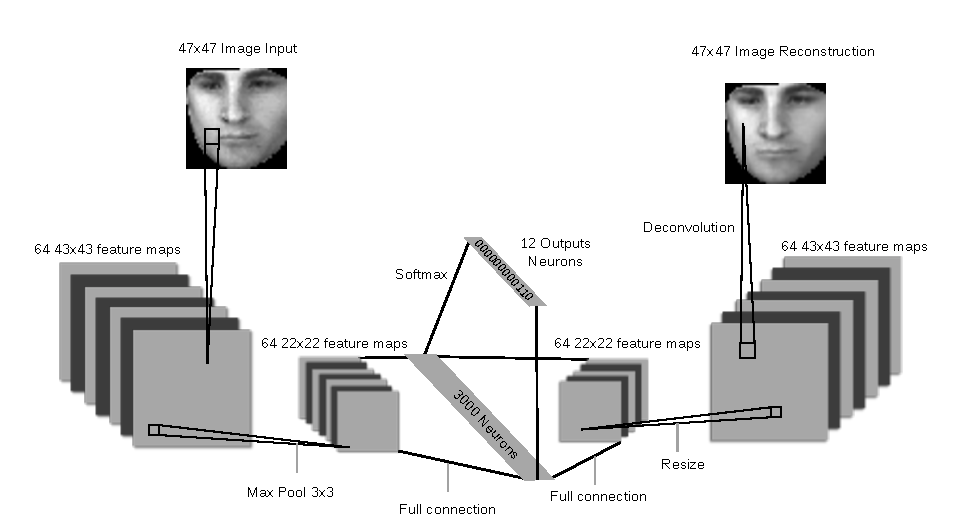
\includegraphics[width=\textwidth]{illustrations/aec_network.pdf}
     \captionof{figure}{General structure of the proposed network. Each rectangle
     represents many layers of neurons and the thin lines represent connections between layers.}
    \end{figure}

    Deep learning is emerging as a powerful tool in modelling a wide range of patterns
    in data, it has been applied to the problem of FAU a number of times and achieved
    good classification rates. One complication which arises when using Deep Neural
    Networks DNNs to classify AUs is that many frames are unlabelled (have neutral expressions)
    and hence the standard supervised DNN do not make good use of this information.
    This project aims to investigate how an autoencoder could be combined with the
    already established deep learning methods related to FAU in order to improve the performance
    of these techniques and better leverage unlabelled data. This unlabelled data may
    come from within the standard AU datasets or from larger databases of faces.
    The DISFA dataset is chosen for initial experiments.
  \section{Potential Applications}
  \section{Contributions}
  \section{Thesis Outline}
